% ===========================================================================
%  TikuOS — Memory Management: MPU Write-Protection Wrappers
%  Beamer Presentation
% ===========================================================================
\documentclass[aspectratio=169, 10pt]{beamer}

% ---- Theme ----------------------------------------------------------------
\usetheme{Madrid}
\usecolortheme{whale}
\setbeamertemplate{navigation symbols}{}
\setbeamertemplate{footline}{%
  \leavevmode\hbox{%
    \begin{beamercolorbox}[wd=.33\paperwidth,ht=2.5ex,dp=1ex,center]{author in head/foot}%
      \usebeamerfont{author in head/foot}\insertshortauthor
    \end{beamercolorbox}%
    \begin{beamercolorbox}[wd=.34\paperwidth,ht=2.5ex,dp=1ex,center]{title in head/foot}%
      \usebeamerfont{title in head/foot}\insertshorttitle
    \end{beamercolorbox}%
    \begin{beamercolorbox}[wd=.33\paperwidth,ht=2.5ex,dp=1ex,right]{date in head/foot}%
      \usebeamerfont{date in head/foot}\insertshortdate{}\hspace*{2em}%
      \insertframenumber{}/\inserttotalframenumber\hspace*{2ex}
    \end{beamercolorbox}}%
  \vskip0pt%
}

% ---- Packages -------------------------------------------------------------
\usepackage{listings}
\usepackage{graphicx}
\usepackage{hyperref}
\usepackage{booktabs}
\usepackage{multirow}
\usepackage{tikz}
\usetikzlibrary{arrows.meta, positioning, shapes.geometric, calc, decorations.pathreplacing}

% ---- Code listing style ---------------------------------------------------
\lstset{
  basicstyle=\ttfamily\scriptsize,
  keywordstyle=\color{blue}\bfseries,
  commentstyle=\color{gray},
  stringstyle=\color{red!70!black},
  showstringspaces=false,
  breaklines=true,
  frame=single,
  rulecolor=\color{black!30},
  backgroundcolor=\color{blue!3},
  tabsize=4,
}
\lstdefinestyle{cstyle}{
  language=C,
  morekeywords={uint8_t,uint16_t,uint32_t,tiku_mpu_seg_t,tiku_mpu_perm_t,
                tiku_mpu_write_fn,tiku_mem_err_t,tiku_mem_arch_size_t,
                TIKU_MPU_SEG1,TIKU_MPU_SEG2,TIKU_MPU_SEG3,
                TIKU_MPU_READ,TIKU_MPU_WRITE,TIKU_MPU_EXEC,
                TIKU_MPU_RD_WR,TIKU_MPU_RD_EXEC,TIKU_MPU_ALL,
                TIKU_MEM_OK,NULL},
}
\lstdefinestyle{bashstyle}{
  language=bash,
  morekeywords={sudo,apt,make,gcc},
}

% ---- Metadata -------------------------------------------------------------
\title[TikuOS MPU]{TikuOS MPU Write-Protection Wrappers}
\subtitle{Simple. Ubiquitous. Intelligence, Everywhere.}
\author[Ambuj Varshney]{Ambuj Varshney \\ \texttt{ambuj@tiku-os.org}}
\date{\today}

% ===========================================================================
\begin{document}

% ---------------------------------------------------------------------------
\begin{frame}
\titlepage
\end{frame}

% ---------------------------------------------------------------------------
\begin{frame}{Outline}
\tableofcontents
\end{frame}

% ===========================================================================
\section{Why FRAM Write-Protection?}
% ===========================================================================

\begin{frame}{The Problem: Unprotected FRAM}
\begin{columns}[T]
\begin{column}{0.48\textwidth}
\textbf{Without MPU protection:}
\begin{itemize}
  \item Wild pointers can corrupt FRAM silently
  \item Runaway code can overwrite calibration data
  \item ISR bugs can damage persistent state
  \item Stack overflows can reach FRAM regions
  \item Corruption persists across reboots
\end{itemize}

\vspace{0.5em}
\begin{alertblock}{FRAM Makes It Worse}
Unlike SRAM, FRAM is non-volatile --- a single wild write
persists across power cycles. A corrupted calibration value
stays corrupted until explicitly fixed.
\end{alertblock}
\end{column}

\begin{column}{0.48\textwidth}
\textbf{TikuOS MPU wrappers:}
\begin{itemize}
  \item Default: FRAM is read+execute, \textbf{no write}
  \item Explicit unlock/lock for intentional writes
  \item Scoped write helper disables interrupts
  \item Per-segment permission control
  \item Password-protected hardware registers
  \item Violation detection via NMI
\end{itemize}

\vspace{0.5em}
\begin{block}{Defense in Depth}
The MPU acts as a hardware safety net --- even if software has
a bug, it cannot accidentally modify FRAM without going through
the controlled unlock sequence.
\end{block}
\end{column}
\end{columns}
\end{frame}

% ===========================================================================
\section{MSP430 MPU Hardware}
% ===========================================================================

\begin{frame}{MPU Register Architecture}
\begin{columns}[T]
\begin{column}{0.48\textwidth}
\textbf{Key registers:}

\vspace{0.5em}
\begin{tabular}{@{}lp{5cm}@{}}
\toprule
\textbf{Register} & \textbf{Purpose} \\
\midrule
\texttt{MPUCTL0} & Control: password (upper byte), enable bit, lock bit, SEGIE \\
\texttt{MPUCTL1} & Violation flags (which segment was violated) \\
\texttt{MPUSAM} & Segment Access Mode: R/W/X permissions per segment \\
\texttt{MPUSEGB1/2} & Segment boundary addresses \\
\bottomrule
\end{tabular}

\vspace{0.5em}
\begin{alertblock}{Password Protection}
Every write to \texttt{MPUCTL0} must include \texttt{0xA500} in
the upper byte. Without it, the hardware ignores the write (or
triggers a reset). This prevents wild pointers from accidentally
changing memory protection.
\end{alertblock}
\end{column}

\begin{column}{0.48\textwidth}
\textbf{MPUSAM bit layout:}
\begin{center}
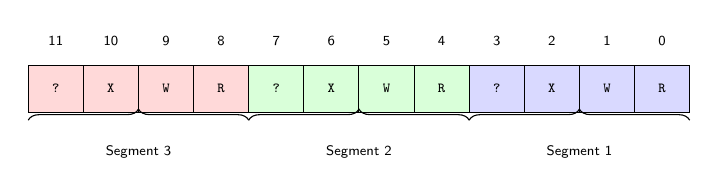
\begin{tikzpicture}[
    cell/.style={draw, minimum width=0.7cm, minimum height=0.6cm,
                 font=\tiny\ttfamily},
    label/.style={font=\tiny\sffamily},
    >=Stealth
  ]
  % Bit numbers
  \foreach \i/\b in {0/11,1/10,2/9,3/8,4/7,5/6,6/5,7/4,8/3,9/2,10/1,11/0} {
    \node[label] at (\i*0.7+0.35, 0.6) {\b};
  }
  % Segment 3 bits
  \foreach \i/\v in {0/?,1/X,2/W,3/R} {
    \node[cell, fill=red!15] at (\i*0.7+0.35, 0) {\v};
  }
  % Segment 2 bits
  \foreach \i/\v in {4/?,5/X,6/W,7/R} {
    \node[cell, fill=green!15] at (\i*0.7+0.35, 0) {\v};
  }
  % Segment 1 bits
  \foreach \i/\v in {8/?,9/X,10/W,11/R} {
    \node[cell, fill=blue!15] at (\i*0.7+0.35, 0) {\v};
  }
  % Segment labels
  \draw[decorate, decoration={brace, amplitude=4pt}]
    (0, -0.4) -- (2.8, -0.4) node[midway, below=0.2cm, font=\tiny\sffamily] {Segment 3};
  \draw[decorate, decoration={brace, amplitude=4pt}]
    (2.8, -0.4) -- (5.6, -0.4) node[midway, below=0.2cm, font=\tiny\sffamily] {Segment 2};
  \draw[decorate, decoration={brace, amplitude=4pt}]
    (5.6, -0.4) -- (8.4, -0.4) node[midway, below=0.2cm, font=\tiny\sffamily] {Segment 1};
\end{tikzpicture}
\end{center}

\vspace{0.3em}
\small
Each segment has 3 permission bits (R/W/X) in a 4-bit nybble.

\vspace{0.3em}
\textbf{Default value \texttt{0x0555}:}\\
\texttt{0x5} = \texttt{0b0101} = R+X (no W) per segment.\\
Three segments: \texttt{0x0555}.

\vspace{0.3em}
\textbf{Unlock value \texttt{0x0222}:}\\
ORing this sets the W bit in all three segments.
\end{column}
\end{columns}
\end{frame}

% ===========================================================================
\section{Architecture \& Types}
% ===========================================================================

\begin{frame}[fragile]{MPU Types (kernel/memory/tiku\_mem.h)}
\begin{columns}[T]
\begin{column}{0.48\textwidth}
\begin{lstlisting}[style=cstyle, title={Segment identifiers}]
typedef enum {
    TIKU_MPU_SEG1 = 0,
    TIKU_MPU_SEG2 = 1,
    TIKU_MPU_SEG3 = 2
} tiku_mpu_seg_t;
\end{lstlisting}

\begin{lstlisting}[style=cstyle, title={Permission flags}]
typedef enum {
    TIKU_MPU_READ    = 0x01,
    TIKU_MPU_WRITE   = 0x02,
    TIKU_MPU_EXEC    = 0x04,
    TIKU_MPU_RD_WR   = 0x03,
    TIKU_MPU_RD_EXEC = 0x05,
    TIKU_MPU_ALL     = 0x07
} tiku_mpu_perm_t;
\end{lstlisting}
\end{column}

\begin{column}{0.48\textwidth}
\begin{lstlisting}[style=cstyle, title={Scoped write callback}]
typedef void (*tiku_mpu_write_fn)(
    void *ctx);
\end{lstlisting}

\vspace{0.5em}
\begin{block}{Design Choices}
\begin{itemize}
  \item Permission flags map directly to hardware bit positions
  \item Compound permissions (\texttt{RD\_WR}, \texttt{RD\_EXEC}) are
        pre-defined for convenience
  \item Callback takes an opaque \texttt{void *ctx} so the caller
        can pass any data without globals
\end{itemize}
\end{block}
\end{column}
\end{columns}
\end{frame}

% ===========================================================================
\section{Platform Layering}
% ===========================================================================

\begin{frame}[fragile]{Three-Layer Architecture}
\begin{center}
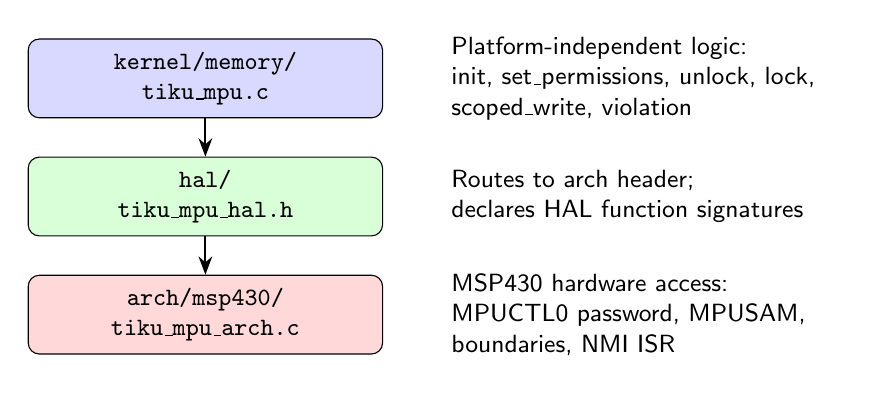
\begin{tikzpicture}[
    box/.style={draw, rounded corners, minimum width=4.5cm, minimum height=1cm,
                font=\small\ttfamily, align=center},
    arrow/.style={->, thick, >=Stealth},
    label/.style={font=\small\sffamily, text width=5cm, align=left}
  ]
  \node[box, fill=blue!15] (kernel) at (0, 3)
    {kernel/memory/\\tiku\_mpu.c};
  \node[box, fill=green!15] (hal) at (0, 1.5)
    {hal/\\tiku\_mpu\_hal.h};
  \node[box, fill=red!15] (arch) at (0, 0)
    {arch/msp430/\\tiku\_mpu\_arch.c};

  \draw[arrow] (kernel) -- (hal);
  \draw[arrow] (hal) -- (arch);

  \node[label, anchor=west] at (3, 3) {Platform-independent logic:\\
    init, set\_permissions, unlock, lock, scoped\_write, violation};
  \node[label, anchor=west] at (3, 1.5) {Routes to arch header;\\
    declares HAL function signatures};
  \node[label, anchor=west] at (3, 0) {MSP430 hardware access:\\
    MPUCTL0 password, MPUSAM, boundaries, NMI ISR};
\end{tikzpicture}
\end{center}

\vspace{0.3em}
\begin{block}{Why This Layering?}
The kernel MPU code (\texttt{tiku\_mpu.c}) contains only delegation
and sequencing logic --- no \texttt{\#include <msp430.h>}, no register names,
no intrinsics. Porting to a new platform means writing a new arch file; the
kernel code stays untouched.
\end{block}
\end{frame}

% ---------------------------------------------------------------------------
\begin{frame}[fragile]{HAL Interface}
\begin{columns}[T]
\begin{column}{0.48\textwidth}
\begin{lstlisting}[style=cstyle, title={hal/tiku\_mpu\_hal.h --- Low-level}]
/* Read/write segment-access register */
uint16_t tiku_mpu_arch_get_sam(void);
void tiku_mpu_arch_set_sam(uint16_t sam);

/* Read MPU control register */
uint16_t tiku_mpu_arch_get_ctl(void);

/* Interrupt control */
void tiku_mpu_arch_disable_irq(void);
void tiku_mpu_arch_enable_irq(void);
\end{lstlisting}
\end{column}

\begin{column}{0.48\textwidth}
\begin{lstlisting}[style=cstyle, title={hal/tiku\_mpu\_hal.h --- Higher-level}]
/* Configure segment boundaries */
void tiku_mpu_arch_init_segments(void);

/* Set default R+X protection */
void tiku_mpu_arch_set_default_protection(void);

/* Per-segment permissions */
void tiku_mpu_arch_set_seg_perm(
    uint8_t seg, uint8_t perm);

/* NVM unlock/lock (all segments) */
uint16_t tiku_mpu_arch_unlock_nvm(void);
void tiku_mpu_arch_lock_nvm(
    uint16_t saved_state);

/* Violation detection */
void tiku_mpu_arch_enable_violation_nmi(void);
uint16_t tiku_mpu_arch_get_violation_flags(void);
void tiku_mpu_arch_clear_violation_flags(void);
\end{lstlisting}
\end{column}
\end{columns}

\vspace{0.3em}
\begin{block}{Kernel Calls HAL}
The kernel never writes to hardware registers directly.
All register access, password handling, and bit manipulation
is encapsulated in the arch layer.
\end{block}
\end{frame}

% ---------------------------------------------------------------------------
\begin{frame}[fragile]{MSP430 Arch Implementation}
\begin{lstlisting}[style=cstyle, title={arch/msp430/tiku\_mpu\_arch.c}]
#include "tiku_mpu_arch.h"
#include <msp430.h>

void tiku_mpu_arch_init_segments(void) {
    MPUCTL0  = MPUPW;                              /* Unlock config */
    MPUSEGB1 = TIKU_DEVICE_MPU_SEG2_START >> 4;    /* Segment 2 boundary */
    MPUSEGB2 = TIKU_DEVICE_MPU_SEG3_START >> 4;    /* Segment 3 boundary */
    MPUCTL0  = MPUPW | MPUENA;                     /* Re-enable MPU */
}

void tiku_mpu_arch_set_sam(uint16_t sam) {
    uint16_t flags = MPUCTL0 & MPUSEGIE;  /* Preserve violation NMI enable */
    MPUCTL0 = MPUPW;                       /* Unlock with password (0xA500) */
    MPUSAM  = sam;                          /* Set new permissions */
    MPUCTL0 = MPUPW | MPUENA | flags;     /* Re-enable + preserved flags */
}

void tiku_mpu_arch_disable_irq(void) { __disable_interrupt(); }
void tiku_mpu_arch_enable_irq(void)  { __enable_interrupt(); }
\end{lstlisting}

\vspace{0.3em}
\begin{alertblock}{All Hardware Access in One File}
The password (\texttt{MPUPW}), enable bit (\texttt{MPUENA}), segment
boundaries, NMI configuration, and MSP430 intrinsics are confined to this
single arch file. The \texttt{MPUSEGIE} flag is preserved across
\texttt{set\_sam()} calls so that enabling violation detection is not
accidentally undone by a later permission change.
\end{alertblock}
\end{frame}

% ===========================================================================
\section{API Reference}
% ===========================================================================

\begin{frame}[fragile]{tiku\_mpu\_init()}
\begin{lstlisting}[style=cstyle]
void tiku_mpu_init(void);
\end{lstlisting}

\begin{itemize}
  \item Configures MPU segment boundaries, then sets all three segments to \textbf{read + execute, no write}
  \item Called by \texttt{tiku\_mem\_init()} at boot --- first thing before any other subsystem
  \item After this call, any attempt to write to FRAM triggers an MPU violation
\end{itemize}

\vspace{0.3em}
\begin{lstlisting}[style=cstyle, title={kernel/memory/tiku\_mpu.c}]
void tiku_mpu_init(void) {
    tiku_mpu_arch_init_segments();           /* Set up segment boundaries */
    tiku_mpu_arch_set_default_protection();  /* R+X on all 3 segments (0x0555) */
}
\end{lstlisting}

\vspace{0.3em}
\begin{block}{Boot Sequence}
\texttt{tiku\_mem\_init()} calls \texttt{tiku\_mpu\_init()} first, then
\texttt{tiku\_mem\_arch\_init()}. Segment boundaries are configured before
protection is applied, and FRAM is write-protected before any other
memory subsystem initialization runs.
\end{block}
\end{frame}

% ---------------------------------------------------------------------------
\begin{frame}[fragile]{tiku\_mpu\_unlock\_nvm() / tiku\_mpu\_lock\_nvm()}
\begin{columns}[T]
\begin{column}{0.48\textwidth}
\begin{lstlisting}[style=cstyle, title={Unlock: enable writes}]
uint16_t tiku_mpu_unlock_nvm(void)
{
    return tiku_mpu_arch_unlock_nvm();
}
\end{lstlisting}

\begin{lstlisting}[style=cstyle, title={Arch implementation}]
uint16_t tiku_mpu_arch_unlock_nvm(void)
{
    uint16_t saved =
        tiku_mpu_arch_get_sam();

    tiku_mpu_arch_set_sam(
        saved | 0x0222);

    return saved;
}
\end{lstlisting}

\begin{itemize}
  \item Saves current SAM state
  \item ORs in write bit for all segments
  \item Returns saved state for later restore
\end{itemize}
\end{column}

\begin{column}{0.48\textwidth}
\begin{lstlisting}[style=cstyle, title={Lock: restore state}]
void tiku_mpu_lock_nvm(
    uint16_t saved_state)
{
    tiku_mpu_arch_lock_nvm(saved_state);
}
\end{lstlisting}

\begin{lstlisting}[style=cstyle, title={Arch implementation}]
void tiku_mpu_arch_lock_nvm(
    uint16_t saved_state)
{
    tiku_mpu_arch_set_sam(saved_state);
}
\end{lstlisting}

\begin{itemize}
  \item Restores SAM to pre-unlock value
  \item Removes write permission
  \item Safe to call when already locked
\end{itemize}

\vspace{0.5em}
\begin{block}{Usage Pattern}
\texttt{saved = tiku\_mpu\_unlock\_nvm();}\\
\texttt{// ... write to FRAM ...}\\
\texttt{tiku\_mpu\_lock\_nvm(saved);}
\end{block}
\end{column}
\end{columns}
\end{frame}

% ---------------------------------------------------------------------------
\begin{frame}[fragile]{tiku\_mpu\_scoped\_write()}
\begin{lstlisting}[style=cstyle]
void tiku_mpu_scoped_write(tiku_mpu_write_fn fn, void *ctx);
\end{lstlisting}

\begin{lstlisting}[style=cstyle, title={kernel/memory/tiku\_mpu.c}]
void tiku_mpu_scoped_write(tiku_mpu_write_fn fn, void *ctx) {
    uint16_t saved;

    tiku_mpu_arch_disable_irq();   /* 1. Disable interrupts */
    saved = tiku_mpu_unlock_nvm(); /* 2. Unlock NVM */

    fn(ctx);                        /* 3. Execute write function */

    tiku_mpu_lock_nvm(saved);      /* 4. Relock NVM */
    tiku_mpu_arch_enable_irq();    /* 5. Re-enable interrupts */
}
\end{lstlisting}

\vspace{0.3em}
\begin{columns}[T]
\begin{column}{0.48\textwidth}
\begin{alertblock}{Why Disable Interrupts?}
While NVM is unlocked, any ISR has write access.
A bug in an ISR could corrupt persistent data.
Disabling interrupts ensures only the caller's
function writes to NVM.
\end{alertblock}
\end{column}
\begin{column}{0.48\textwidth}
\begin{alertblock}{Keep It Short}
While interrupts are disabled, hardware events
queue up. The write function must be brief ---
long operations should be split across multiple
\texttt{scoped\_write} calls.
\end{alertblock}
\end{column}
\end{columns}
\end{frame}

% ---------------------------------------------------------------------------
\begin{frame}[fragile]{tiku\_mpu\_set\_permissions()}
\begin{lstlisting}[style=cstyle]
void tiku_mpu_set_permissions(tiku_mpu_seg_t seg, tiku_mpu_perm_t perm);
\end{lstlisting}

\begin{lstlisting}[style=cstyle, title={kernel/memory/tiku\_mpu.c --- delegates to arch}]
void tiku_mpu_set_permissions(tiku_mpu_seg_t seg, tiku_mpu_perm_t perm) {
    tiku_mpu_arch_set_seg_perm((uint8_t)seg, (uint8_t)perm);
}
\end{lstlisting}

\begin{lstlisting}[style=cstyle, title={arch/msp430/tiku\_mpu\_arch.c --- register manipulation}]
void tiku_mpu_arch_set_seg_perm(uint8_t seg, uint8_t perm) {
    uint16_t shift = (uint16_t)seg * 4U;
    uint16_t mask  = (uint16_t)0x07 << shift;
    uint16_t sam   = tiku_mpu_arch_get_sam();

    sam = (sam & ~mask) | (((uint16_t)perm & 0x07) << shift);
    tiku_mpu_arch_set_sam(sam);
}
\end{lstlisting}

\vspace{0.3em}
\begin{itemize}
  \item Modifies only the targeted segment's 3-bit permission field
  \item Other segments are left untouched
  \item All SAM bit manipulation is in the arch layer --- kernel just delegates
\end{itemize}

\vspace{0.3em}
\textbf{Example:} Make segment 3 writable while keeping segments 1--2 locked:
\begin{lstlisting}[style=cstyle]
tiku_mpu_set_permissions(TIKU_MPU_SEG3, TIKU_MPU_RD_WR);
/* ... write to segment 3 FRAM region ... */
tiku_mpu_set_permissions(TIKU_MPU_SEG3, TIKU_MPU_RD_EXEC);
\end{lstlisting}
\end{frame}

% ---------------------------------------------------------------------------
\begin{frame}[fragile]{Violation Detection}
\begin{columns}[T]
\begin{column}{0.48\textwidth}
\begin{lstlisting}[style=cstyle, title={kernel/memory/tiku\_mpu.c}]
void tiku_mpu_enable_violation_nmi(void)
{
    tiku_mpu_arch_enable_violation_nmi();
}

uint16_t tiku_mpu_get_violation_flags(void)
{
    return
      tiku_mpu_arch_get_violation_flags();
}

void tiku_mpu_clear_violation_flags(void)
{
    tiku_mpu_arch_clear_violation_flags();
}
\end{lstlisting}

\begin{block}{Usage Pattern}
\texttt{tiku\_mpu\_enable\_violation\_nmi();}\\
\texttt{tiku\_mpu\_clear\_violation\_flags();}\\
\texttt{// ... code that may violate ...}\\
\texttt{flags = tiku\_mpu\_get\_violation\_flags();}
\end{block}
\end{column}

\begin{column}{0.48\textwidth}
\begin{lstlisting}[style=cstyle, title={arch/msp430/tiku\_mpu\_arch.c}]
static volatile uint16_t
    latched_violation_flags;

void tiku_mpu_arch_enable_violation_nmi(void)
{
    MPUCTL0 = MPUPW | MPUENA | MPUSEGIE;
}

/* SYSNMI ISR --- latch flags before
   SYSSNIV read clears them */
TIKU_ISR(SYSNMI_VECTOR,
         tiku_mpu_sysnmi_isr)
{
    latched_violation_flags |= MPUCTL1;
    (void)SYSSNIV; /* acknowledge NMI */
}
\end{lstlisting}

\begin{alertblock}{Why NMI Instead of Reset?}
By default, an MPU violation causes a device reset, losing all
state. Setting \texttt{MPUSEGIE} switches to an NMI, allowing
the CPU to continue and software to inspect which segment was
violated.
\end{alertblock}
\end{column}
\end{columns}
\end{frame}

% ===========================================================================
\section{Usage Examples}
% ===========================================================================

\begin{frame}{When to Use MPU Protection}
\begin{columns}[T]
\begin{column}{0.48\textwidth}
\begin{block}{MPU Protection IS Right When\ldots}
\begin{itemize}
  \item Calibration data in FRAM must survive bugs
  \item ISRs run alongside FRAM-writing code
  \item Persistent state must not be silently corrupted
  \item You want hardware-enforced access control
  \item You need to diagnose wild-pointer bugs
\end{itemize}
\end{block}
\end{column}

\begin{column}{0.48\textwidth}
\begin{alertblock}{MPU Protection Is NOT Needed When\ldots}
\begin{itemize}
  \item All data lives in SRAM (volatile anyway)
  \item Only one task ever writes to FRAM
  \item You are prototyping and not yet hardening
  \item The MCU has no MPU (some MSP430 variants)
\end{itemize}
\end{alertblock}
\end{column}
\end{columns}

\vspace{0.5em}
\begin{block}{Rule of Thumb}
If you store anything in FRAM that must be correct after the next reboot ---
calibration, configuration, boot counter --- protect it with the MPU.
The cost is a few cycles per write; the benefit is catching bugs that
would otherwise cause silent, persistent corruption.
\end{block}
\end{frame}

% ---------------------------------------------------------------------------
\begin{frame}[fragile]{Example 1: The Bug MPU Catches}
\begin{columns}[T]
\begin{column}{0.48\textwidth}
\begin{lstlisting}[style=cstyle, title={Without MPU --- silent corruption}]
/* Calibration stored in FRAM */
static uint16_t __attribute__((
    section(".persistent")))
    adc_offset = 42;

/* Bug: uninitialized pointer in ISR */
void __attribute__((interrupt))
TIMER_ISR(void)
{
    uint16_t *p;  /* uninitialised! */
    *p = 0xFFFF;  /* wild write */
    /* If p happens to point at
       adc_offset, calibration is
       silently destroyed.
       Persists across reboots. */
}
\end{lstlisting}
\end{column}

\begin{column}{0.48\textwidth}
\begin{lstlisting}[style=cstyle, title={With MPU --- fault caught instantly}]
/* Same bug, but MPU is enabled */
void __attribute__((interrupt))
TIMER_ISR(void)
{
    uint16_t *p;  /* uninitialised! */
    *p = 0xFFFF;  /* wild write */
    /* MPU detects write to locked
       FRAM segment -> triggers NMI
       instead of silent corruption.
       adc_offset remains intact. */
}
\end{lstlisting}

\vspace{0.3em}
\begin{alertblock}{Key Insight}
Without MPU, the bug is invisible --- the device
reboots with wrong calibration and you have no
idea when or how it happened. With MPU, the NMI
fires immediately, giving you the PC value and
the violated segment.
\end{alertblock}
\end{column}
\end{columns}
\end{frame}

% ---------------------------------------------------------------------------
\begin{frame}[fragile]{Example 2: Scoped Write for Sensor Calibration}
\begin{lstlisting}[style=cstyle]
/* Context for the scoped write callback */
typedef struct {
    tiku_persist_store_t *store;
    const uint8_t *data;
    tiku_mem_arch_size_t len;
} cal_write_ctx_t;

static void write_cal(void *arg) {
    cal_write_ctx_t *ctx = (cal_write_ctx_t *)arg;
    tiku_persist_write(ctx->store, "cal", ctx->data, ctx->len);
}

void save_calibration(tiku_persist_store_t *store,
                       const uint8_t *cal_data, tiku_mem_arch_size_t len)
{
    cal_write_ctx_t ctx = { store, cal_data, len };

    /* scoped_write: disable IRQ -> unlock NVM -> write -> lock -> enable IRQ */
    tiku_mpu_scoped_write(write_cal, &ctx);
}
\end{lstlisting}

\vspace{0.3em}
\begin{block}{Safety Guarantees}
NVM is writable only during the \texttt{write\_cal} callback.
Interrupts are disabled so no ISR can interfere. After return,
NVM is write-protected again automatically.
\end{block}
\end{frame}

% ---------------------------------------------------------------------------
\begin{frame}[fragile]{Example 3: Per-Segment Protection Policies}
\begin{columns}[T]
\begin{column}{0.48\textwidth}
\begin{lstlisting}[style=cstyle, title={Bootloader vs application FRAM}]
/* Segment 1: bootloader code (FRAM)
     -> read + execute, NEVER write
   Segment 2: application code (FRAM)
     -> read + execute, no write
   Segment 3: persistent data (FRAM)
     -> read + write (controlled) */

void boot_mpu_setup(void) {
    tiku_mpu_init();  /* all R+X */

    /* Seg 1: bootloader is immutable
       (even scoped_write won't help) */
    tiku_mpu_set_permissions(
        TIKU_MPU_SEG1, TIKU_MPU_RD_EXEC);

    /* Seg 3: data segment gets R+W
       so persist_write can work */
    tiku_mpu_set_permissions(
        TIKU_MPU_SEG3, TIKU_MPU_RD_WR);
}
\end{lstlisting}
\end{column}

\begin{column}{0.48\textwidth}
\begin{lstlisting}[style=cstyle, title={Tighten after init completes}]
void app_start(void) {
    /* During init, seg 3 was R+W
       for persist_register/write.
       Now lock it down. */
    tiku_mpu_set_permissions(
        TIKU_MPU_SEG3, TIKU_MPU_READ);

    /* From here on, only scoped_write
       can write to segment 3.
       Segments 1 and 2 remain R+X
       throughout. */
}
\end{lstlisting}

\vspace{0.3em}
\begin{block}{Why Per-Segment?}
A sensor node's bootloader must never be
overwritten --- even by kernel code.
Separating bootloader, application, and
data into different segments with
independent permissions gives defense
in depth.
\end{block}
\end{column}
\end{columns}
\end{frame}

% ---------------------------------------------------------------------------
\begin{frame}[fragile]{Example 4: Violation Detection for Debugging}
\begin{lstlisting}[style=cstyle]
void debug_mpu_setup(void) {
    tiku_mpu_init();
    tiku_mpu_enable_violation_nmi();   /* NMI instead of reset on violation */
    tiku_mpu_clear_violation_flags();
}

/* Call periodically or after suspicious behaviour */
void check_for_violations(void) {
    uint16_t flags = tiku_mpu_get_violation_flags();
    if (flags != 0) {
        /* Which segment was violated?
           Bit 0 = seg 1, bit 1 = seg 2, bit 2 = seg 3 */
        if (flags & 0x01) uart_puts("SEG1 violated (bootloader region!)\r\n");
        if (flags & 0x02) uart_puts("SEG2 violated (app code region)\r\n");
        if (flags & 0x04) uart_puts("SEG3 violated (data region)\r\n");

        tiku_mpu_clear_violation_flags();
    }
}
\end{lstlisting}

\vspace{0.3em}
\begin{alertblock}{Development vs Production}
During development, enable violation NMI and log which segment was hit ---
this pinpoints wild-pointer bugs immediately. In production, you may
prefer the default behaviour (device reset on violation) to guarantee
a known-good restart rather than continuing with a potentially
corrupted state.
\end{alertblock}
\end{frame}

% ---------------------------------------------------------------------------
\begin{frame}[fragile]{Example 5: Manual Unlock for Batched Writes}
\begin{lstlisting}[style=cstyle]
void batch_persist_update(tiku_persist_store_t *store) {
    uint16_t saved;
    uint8_t cfg_data[] = {0x01, 0x02};
    uint8_t cal_data[] = {0xAA, 0xBB, 0xCC};

    /* Batch multiple NVM writes in one unlock window */
    saved = tiku_mpu_unlock_nvm();

    tiku_persist_write(store, "cfg", cfg_data, sizeof(cfg_data));
    tiku_persist_write(store, "cal", cal_data, sizeof(cal_data));

    tiku_mpu_lock_nvm(saved);
}
\end{lstlisting}

\vspace{0.3em}
\begin{columns}[T]
\begin{column}{0.48\textwidth}
\begin{alertblock}{Trade-off: Batching vs Safety}
Manual unlock/lock avoids per-write overhead but
leaves NVM unprotected for longer. Use
\texttt{scoped\_write} for single writes; manual
unlock for known-safe batches.
\end{alertblock}
\end{column}
\begin{column}{0.48\textwidth}
\begin{block}{When to Batch}
\begin{itemize}
  \item Writing config + calibration together
  \item Initial provisioning at factory
  \item Firmware update writing multiple keys
  \item Any case where all writes are in one function
\end{itemize}
\end{block}
\end{column}
\end{columns}
\end{frame}

% ===========================================================================
\section{File Organization}
% ===========================================================================

\begin{frame}[fragile]{Module File Organization}
\begin{table}
\centering
\small
\begin{tabular}{@{}lll@{}}
\toprule
\textbf{Layer} & \textbf{File} & \textbf{Role} \\
\midrule
\multirow{3}{*}{Kernel (portable)}
  & \texttt{kernel/memory/tiku\_mem.h}  & Unified API: arena + persist + MPU types \\
  & \texttt{kernel/memory/tiku\_mem.c}  & Arena allocator, module init \\
  & \texttt{kernel/memory/tiku\_mpu.c}  & MPU logic: init, unlock, lock, scoped write \\
\midrule
\multirow{2}{*}{HAL}
  & \texttt{hal/tiku\_mem\_hal.h}  & Routes to arch memory header \\
  & \texttt{hal/tiku\_mpu\_hal.h}  & Routes to arch MPU header \\
\midrule
\multirow{2}{*}{Arch (MSP430)}
  & \texttt{arch/msp430/tiku\_mpu\_arch.h} & MPU arch function declarations \\
  & \texttt{arch/msp430/tiku\_mpu\_arch.c} & MPUCTL0/MPUSAM access, boundaries, NMI ISR \\
\midrule
\multirow{2}{*}{Tests}
  & \texttt{tests/memory/test\_mem\_mpu.c}    & 11 MPU test cases \\
  & \texttt{tests/memory/test\_mem\_common.c} & Host stubs + test main \\
\bottomrule
\end{tabular}
\end{table}

\vspace{0.5em}
\begin{block}{Porting to a New Architecture}
Only the arch files change:
\begin{enumerate}
  \item Implement segment boundary setup and default protection
  \item Implement \texttt{set\_seg\_perm()}, \texttt{unlock\_nvm()}, \texttt{lock\_nvm()} for your MPU
  \item Implement \texttt{disable\_irq()} / \texttt{enable\_irq()} for your interrupt controller
  \item The kernel MPU logic and all tests remain untouched
\end{enumerate}
\end{block}
\end{frame}

% ===========================================================================
\section{API Summary}
% ===========================================================================

\begin{frame}{API at a Glance}
\begin{table}
\centering
\small
\begin{tabular}{@{}llll@{}}
\toprule
\textbf{Function} & \textbf{Returns} & \textbf{Complexity} & \textbf{Description} \\
\midrule
\texttt{tiku\_mpu\_init}       & \texttt{void}     & O(1) & Set boundaries + default protection \\
\texttt{tiku\_mpu\_set\_permissions} & \texttt{void} & O(1) & Set permissions on one segment \\
\texttt{tiku\_mpu\_unlock\_nvm}   & \texttt{uint16\_t} & O(1) & Enable writes, return saved state \\
\texttt{tiku\_mpu\_lock\_nvm}    & \texttt{void}     & O(1) & Restore saved protection state \\
\texttt{tiku\_mpu\_scoped\_write} & \texttt{void}     & O(1)+fn & IRQ-safe unlock/write/lock \\
\texttt{tiku\_mpu\_enable\_violation\_nmi} & \texttt{void} & O(1) & Switch violations to NMI \\
\texttt{tiku\_mpu\_get\_violation\_flags} & \texttt{uint16\_t} & O(1) & Read per-segment violation flags \\
\texttt{tiku\_mpu\_clear\_violation\_flags} & \texttt{void} & O(1) & Reset violation flags \\
\bottomrule
\end{tabular}
\end{table}

\vspace{0.5em}
\begin{columns}[T]
\begin{column}{0.48\textwidth}
\begin{block}{Safety Guarantees}
\begin{itemize}
  \item NVM write-protected by default
  \item Hardware password prevents accidental unlock
  \item Scoped write disables interrupts
  \item Lock/unlock are idempotent
  \item MPUSEGIE preserved across set\_sam calls
\end{itemize}
\end{block}
\end{column}
\begin{column}{0.48\textwidth}
\begin{block}{Design Choices}
\begin{itemize}
  \item Platform-independent kernel code
  \item All register access in arch layer
  \item HAL routes to correct platform
  \item Host-testable with stub registers
  \item Violation detection via latched flags
\end{itemize}
\end{block}
\end{column}
\end{columns}
\end{frame}

% ===========================================================================
\section{Test Suite}
% ===========================================================================

\begin{frame}[fragile]{Test Configuration}
\begin{columns}[T]
\begin{column}{0.48\textwidth}
\textbf{Host-native (no hardware):}
\begin{lstlisting}[style=bashstyle]
gcc -std=c99 -Wall -Wextra -I. \
  tests/memory/test_mem_common.c \
  tests/memory/test_mem_mpu.c \
  kernel/memory/tiku_mpu.c \
  -o test_tiku_mpu \
  && ./test_tiku_mpu
\end{lstlisting}

\vspace{0.3em}
Host mode provides stub implementations of all HAL functions ---
plain variables mimic MPU registers so the test can inspect
resulting state without hardware.
\end{column}

\begin{column}{0.48\textwidth}
\begin{lstlisting}[style=cstyle, title={Host HAL stubs in test\_mem\_common.c}]
static uint16_t stub_mpusam;

void tiku_mpu_arch_set_sam(uint16_t sam)
{
    stub_mpuctl0 = 0xA500;
    stub_mpusam  = sam;
    stub_mpuctl0 = 0xA500 | 0x0001;
}

void tiku_mpu_arch_set_default_protection(void)
{ tiku_mpu_arch_set_sam(0x0555); }

uint16_t tiku_mpu_arch_unlock_nvm(void) {
    uint16_t saved = stub_mpusam;
    tiku_mpu_arch_set_sam(saved | 0x0222);
    return saved;
}

/* Violation stub: check SAM bits */
void test_mpu_trigger_seg_violation(
    tiku_mpu_seg_t seg) { /* ... */ }
\end{lstlisting}
\end{column}
\end{columns}
\end{frame}

% ---------------------------------------------------------------------------
\begin{frame}{MPU Test Cases}
\begin{table}
\centering
\small
\begin{tabular}{@{}clp{7.5cm}@{}}
\toprule
\textbf{\#} & \textbf{Test Name} & \textbf{What It Verifies} \\
\midrule
21 & Init defaults       & SAM = 0x0555 (all R+X); CTL enable bit set \\
22 & Unlock / Lock       & Unlock returns saved state (0x0555); SAM becomes 0x0777;
                           lock restores 0x0555 \\
23 & Set permissions     & Changing one segment leaves others untouched \\
24 & Scoped write        & Callback invoked with write bits set; SAM relocked after return \\
25 & Idempotency         & Lock when locked is no-op; double unlock returns correct states \\
26 & All segments        & Set each segment independently; changing one preserves others \\
27 & Permission flags    & Each \texttt{TIKU\_MPU\_*} enum maps to correct SAM bits \\
28 & Re-init restores    & Custom permissions wiped by re-init to default 0x0555 \\
29 & Unlock custom base  & Unlock with non-default base preserves R/X bits, adds W \\
30 & Scoped write custom & Scoped write with custom base permissions works correctly \\
31 & Violation detection & Write to locked segment sets flag; unlocked write does not \\
\bottomrule
\end{tabular}
\end{table}
\end{frame}

% ---------------------------------------------------------------------------
\begin{frame}[fragile]{Test Deep Dive: Scoped Write}
\begin{lstlisting}[style=cstyle, title={test\_mem\_mpu.c --- Scoped write test}]
typedef struct {
    int called;
    uint16_t sam_during;
} scoped_write_ctx_t;

static void scoped_write_cb(void *arg) {
    scoped_write_ctx_t *ctx = (scoped_write_ctx_t *)arg;
    ctx->called = 1;
    ctx->sam_during = tiku_mpu_arch_get_sam();  /* capture state during write */
}

void test_mpu_scoped_write(void) {
    scoped_write_ctx_t ctx = { 0, 0 };

    tiku_mpu_init();
    tiku_mpu_scoped_write(scoped_write_cb, &ctx);

    TEST_ASSERT(ctx.called == 1);                       /* callback was invoked */
    TEST_ASSERT((ctx.sam_during & 0x0222) == 0x0222);   /* write bits set during */
    TEST_ASSERT(tiku_mpu_arch_get_sam() == 0x0555);     /* locked after return */
}
\end{lstlisting}

\vspace{0.3em}
\begin{block}{What This Proves}
The test captures the SAM register \emph{inside} the callback, proving
that NVM was unlocked during execution. After return, SAM is verified
to be relocked --- confirming the full unlock/write/lock sequence works.
\end{block}
\end{frame}

% ---------------------------------------------------------------------------
\begin{frame}[fragile]{Test Deep Dive: Violation Detection}
\begin{lstlisting}[style=cstyle, title={test\_mem\_mpu.c --- Violation detection test}]
void test_mpu_violation_detect(void) {
    tiku_mpu_init();
    tiku_mpu_enable_violation_nmi();
    tiku_mpu_clear_violation_flags();

    TEST_ASSERT(tiku_mpu_get_violation_flags() == 0);    /* clean baseline */

    /* Phase 1: write while locked -> violation flag set */
    test_mpu_trigger_seg_violation(TIKU_MPU_SEG1);       /* host stub */
    TEST_ASSERT(tiku_mpu_get_violation_flags() != 0);    /* violation detected */

    tiku_mpu_clear_violation_flags();
    TEST_ASSERT(tiku_mpu_get_violation_flags() == 0);    /* flags cleared */

    /* Phase 2: write while unlocked -> no violation */
    saved = tiku_mpu_unlock_nvm();
    tiku_mpu_clear_violation_flags();
    test_mpu_trigger_seg_violation(TIKU_MPU_SEG1);
    TEST_ASSERT(tiku_mpu_get_violation_flags() == 0);    /* no violation */
    tiku_mpu_lock_nvm(saved);
}
\end{lstlisting}

\vspace{0.3em}
\begin{block}{Host vs Hardware}
On MSP430, the test writes to a real FRAM address (e.g.\ \texttt{0x4400}) to
trigger a violation. On the host, \texttt{test\_mpu\_trigger\_seg\_violation()}
checks SAM bits and sets the flag accordingly.
\end{block}
\end{frame}

% ===========================================================================
\section{Summary}
% ===========================================================================

\begin{frame}{Summary}
\begin{columns}[T]
\begin{column}{0.48\textwidth}
\begin{block}{MPU Wrapper Design}
\begin{itemize}
  \item Hardware NVM write-protection
  \item Default: read+execute, no write
  \item Explicit unlock/lock pattern
  \item Scoped write with IRQ protection
  \item Per-segment fine-grained control
  \item Password-protected registers
  \item Violation detection via NMI
  \item Platform-independent kernel code
  \item All hardware access in arch layer
\end{itemize}
\end{block}
\end{column}

\begin{column}{0.48\textwidth}
\begin{block}{Test Coverage}
\begin{itemize}
  \item 11 MPU test cases
  \item Runs on host GCC with stub registers
  \item Covers: init, unlock/lock, per-segment,
        scoped write, idempotency, all flags,
        re-init, custom base, violation detection
\end{itemize}
\end{block}

\vspace{0.3em}
\begin{alertblock}{Part of the Memory Module}
The MPU wrappers extend \texttt{tiku\_mem.h} alongside the arena
allocator and persistent store --- same header, same HAL pattern,
same test binary.
\end{alertblock}
\end{column}
\end{columns}
\end{frame}

% ---------------------------------------------------------------------------
\begin{frame}{Thank You}
\begin{center}
\Large\textbf{TikuOS MPU Write-Protection Wrappers}\\[0.5em]
\normalsize FRAM Safety for Physical AI Endpoints\\[1.5em]

\begin{tabular}{rl}
  Repository: & \url{https://github.com/tikuos/tikuOS} \\
  License:    & Apache 2.0 \\
  API Header: & \texttt{kernel/memory/tiku\_mem.h} \\
  MPU Logic:  & \texttt{kernel/memory/tiku\_mpu.c} \\
  Tests:      & \texttt{tests/memory/test\_mem\_mpu.c} \\
\end{tabular}
\end{center}
\end{frame}

\end{document}
